\chapter{Higher order AGP as a cost function}\label{chap:7_higher_order_agp}

In Ch.~\ref{chap:5_cd_as_costfunc} we discussed the idea of using the \acrref{AGP} operator and its approximations in order to construct cost functions for the optimisation of Hamiltonian paths in parameter space. 

\section{Return to two-spin annealing}

In the previous chapter in Sec.~\ref{sec:5.1_2spin_annealing} we investigated the \acrref{COLD} protocol in the case of a two-spin annealing protocol described by the Hamiltonian given by Eq.~\eqref{eq:two_spin_hamiltonian}, where the system starts close to the state $\ket{\uparrow\uparrow}$ and is driven towards a superposition of all the symmetric states. We will return to this simple example in order to illustrate how the integral and maximum amplitude cost functions given by Eq.~\eqref{eq:COLD_costfunc_integral} and Eq.~\eqref{eq:COLD_costfunc_maximum} respectively behave when used to optimise the Hamiltonian path in parameter space for \acrref{COLD}. 

We will use the same control Hamiltonian as that in Eq.~\eqref{eq:COLD_twospin_controlH} of Sec.~\ref{sec:5.1_2spin_annealing} as well as the same \acrref{FO} and \acrref{SO} operator ans\"{a}tze for the \acrref{LCD} operators (Eq.~\eqref{eq:LCD1st} and Eq.~\eqref{eq:twospin_so_lcd} respectively). The key difference between what was done in Ch.~\ref{chap:6_Applications_fidelity} and what we are aiming to demonstrate here is the use of 
 
\begin{equation}\label{eq:twospin_costfunc_int}
    \begin{aligned}
        C_{I, \gamma}(\tau, \betabb) &= \int_{0}^{\tau} dt^{\prime} |\gamma(\lambda(t^{\prime}), \hbb, \betabb)|\\
        C_{I, \zeta}(\tau, \betabb) &= \int_{0}^{\tau} dt^{\prime} |\zeta(\lambda(t^{\prime}), \hbb, \betabb)|\\
        C_{I, (\gamma + \zeta))}(\tau, \betabb) &= \int_{0}^{\tau} dt^{\prime} \left(|\gamma(\lambda(t^{\prime}), \hbb, \betabb)| + |\zeta(\lambda(t^{\prime}), \hbb, \betabb)|\right)
    \end{aligned}
\end{equation}

\begin{equation}\label{eq:twospin_costfunc_amp}
    \begin{aligned}
        C_{A, \gamma}(\tau, \betabb) &= \max_{t^{\prime} \in [0,\tau]} | \gamma(\lambda(t^{\prime}), \hbb, \betabb)| \\
        C_{A, \zeta}(\tau, \betabb) &= \max_{t^{\prime} \in [0,\tau]} | \zeta(\lambda(t^{\prime}), \hbb, \betabb)| \\
        C_{A, (\gamma + \zeta)}(\tau, \betabb) &= \max_{t^{\prime} \in [0,\tau]} \left(| \gamma(\lambda(t^{\prime}), \hbb, \betabb)| + \zeta(\lambda(t^{\prime}), \hbb, \betabb)| \right)
    \end{aligned}
\end{equation}

\begin{figure}[h]
    \centering
    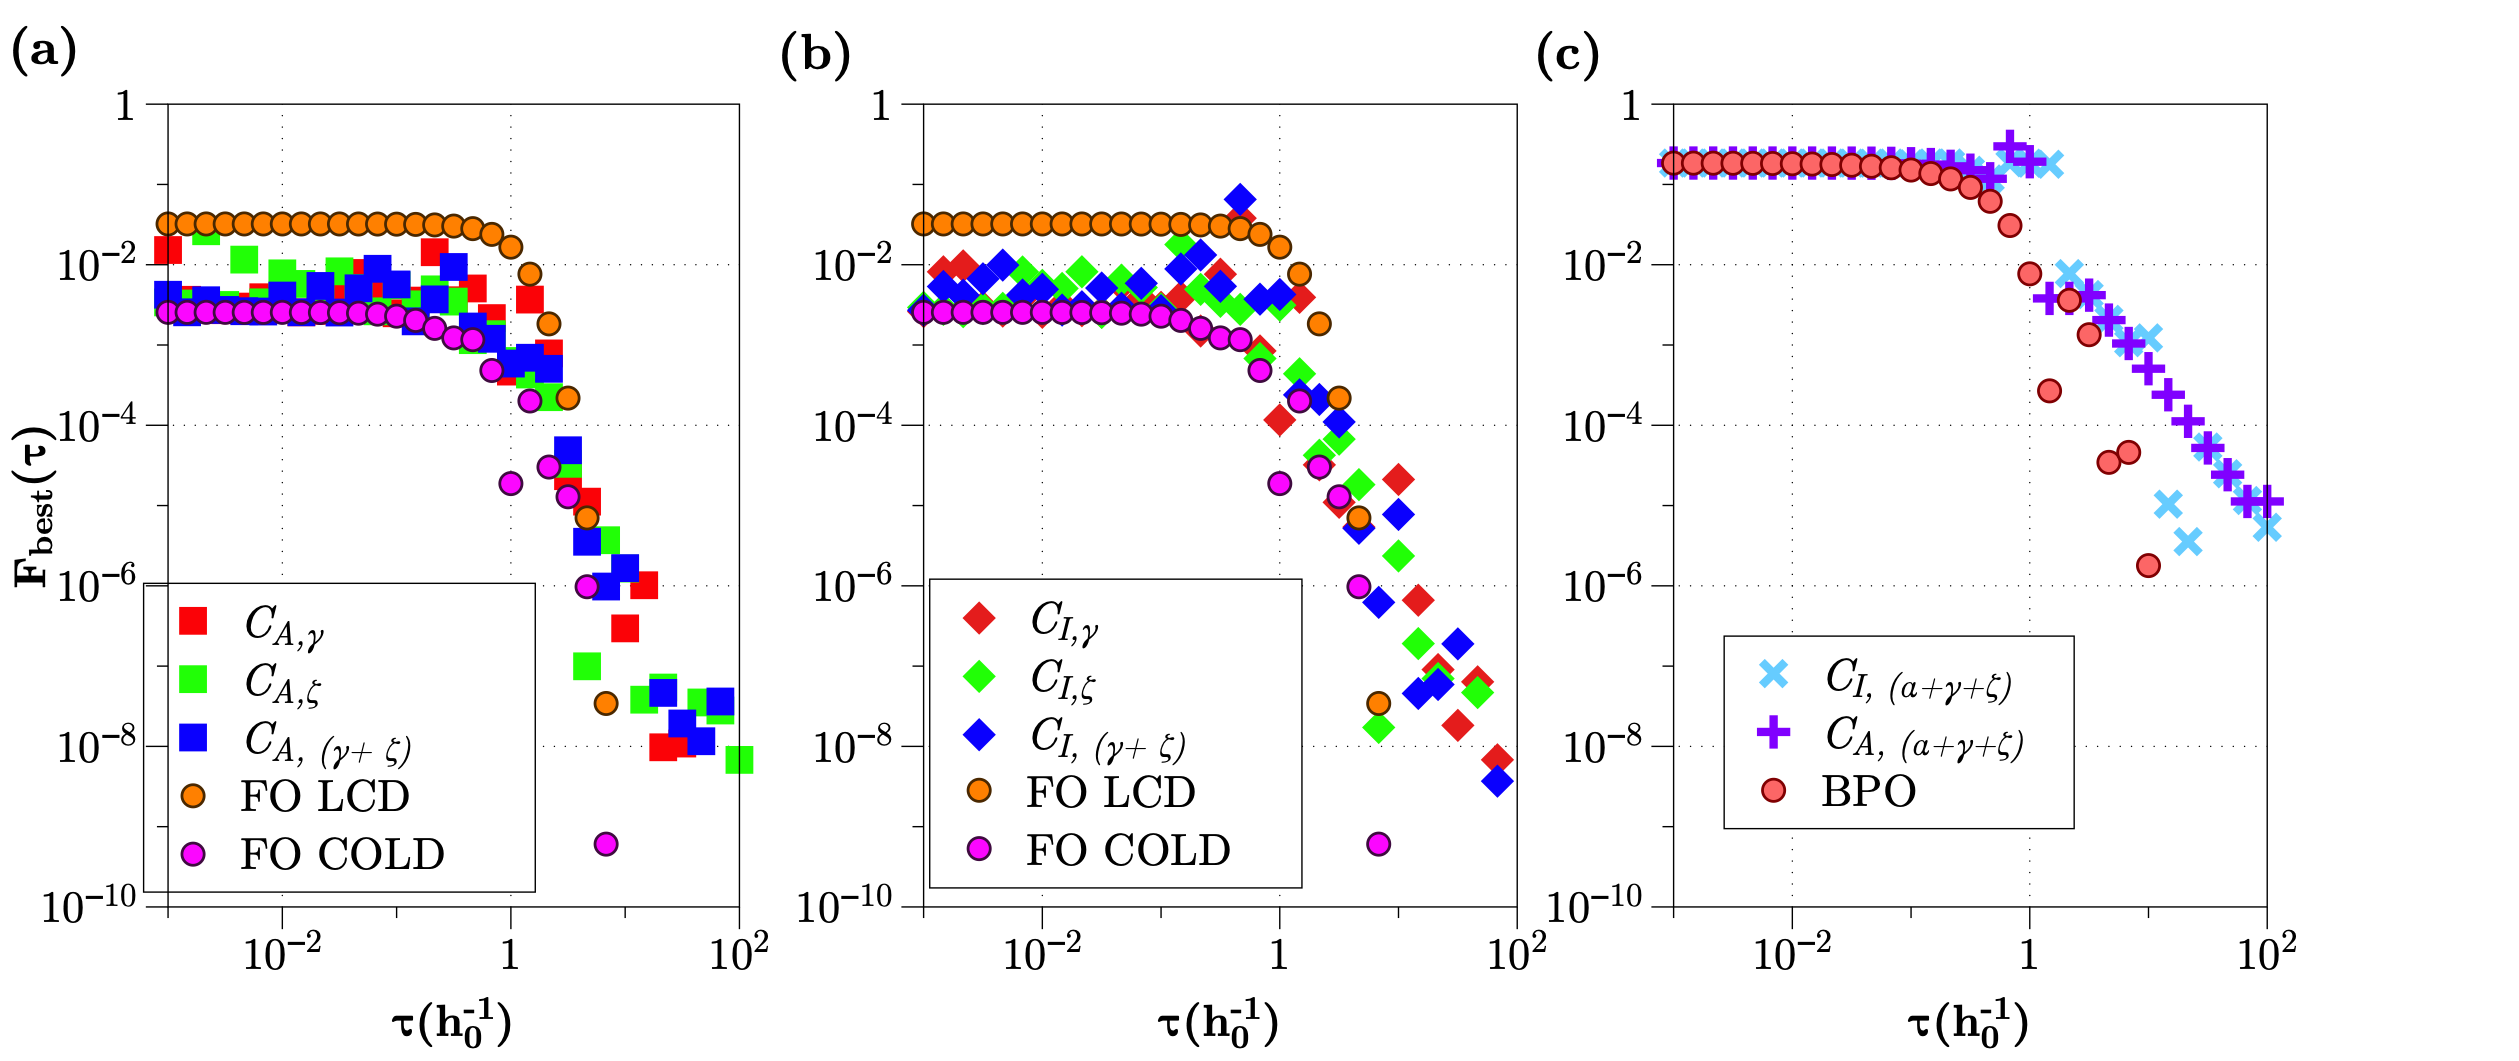
\includegraphics[width=0.8\linewidth]{images/twospin_HO_scatter.png} \caption[Two-spin annealing plots of fidelity versus driving time when minimising different orders of LCD.]{Two-spin annealing plots of fidelity versus driving time when optimising using different cost functions. In both plots, we show the results for \acrref{FO} \acrref{LCD} (orange circles) and \acrref{FO} \acrref{COLD} (pink circles) from Fig.~\ref{fig:twospin_fidelities} for comparison. Then, in (a) we plot the resulting final state fidelities at different driving times $\tau$ obtained when applying \acrref{FO} \acrref{LCD} to control Hamiltonians from Eq.~\eqref{eq:COLD_twospin_controlH} with parameters optimised using the maximum amplitude cost function $C_A$. The results are shown when optimising for $\gamma$ coefficients (red squares, $C_{A, \gamma}$), $\zeta$ coefficients (green squares, $C_{A, \zeta}$) and their sum (blue squares, $C_{A, (\gamma + \zeta)}$). The same is done in (b) for the integral cost function $C_I$, where we plot results in the case of optimising $\gamma$ coefficients (red diamonds, $C_{I, \gamma}$), $\zeta$ coefficients (green diamonds, $C_{I, \zeta}$) and their sum (blue diamonds, $C_{I, (\gamma + \zeta)}$). In all cases, we use $N_k = 1$ parameter and Powell's optimisation method from Sec.~\ref{sec:3.1.3.2_Powell}. The optimisation is done once for each data point.}\label{fig:twospin_scatter}
\end{figure}

\begin{figure}[h]
    \centering
    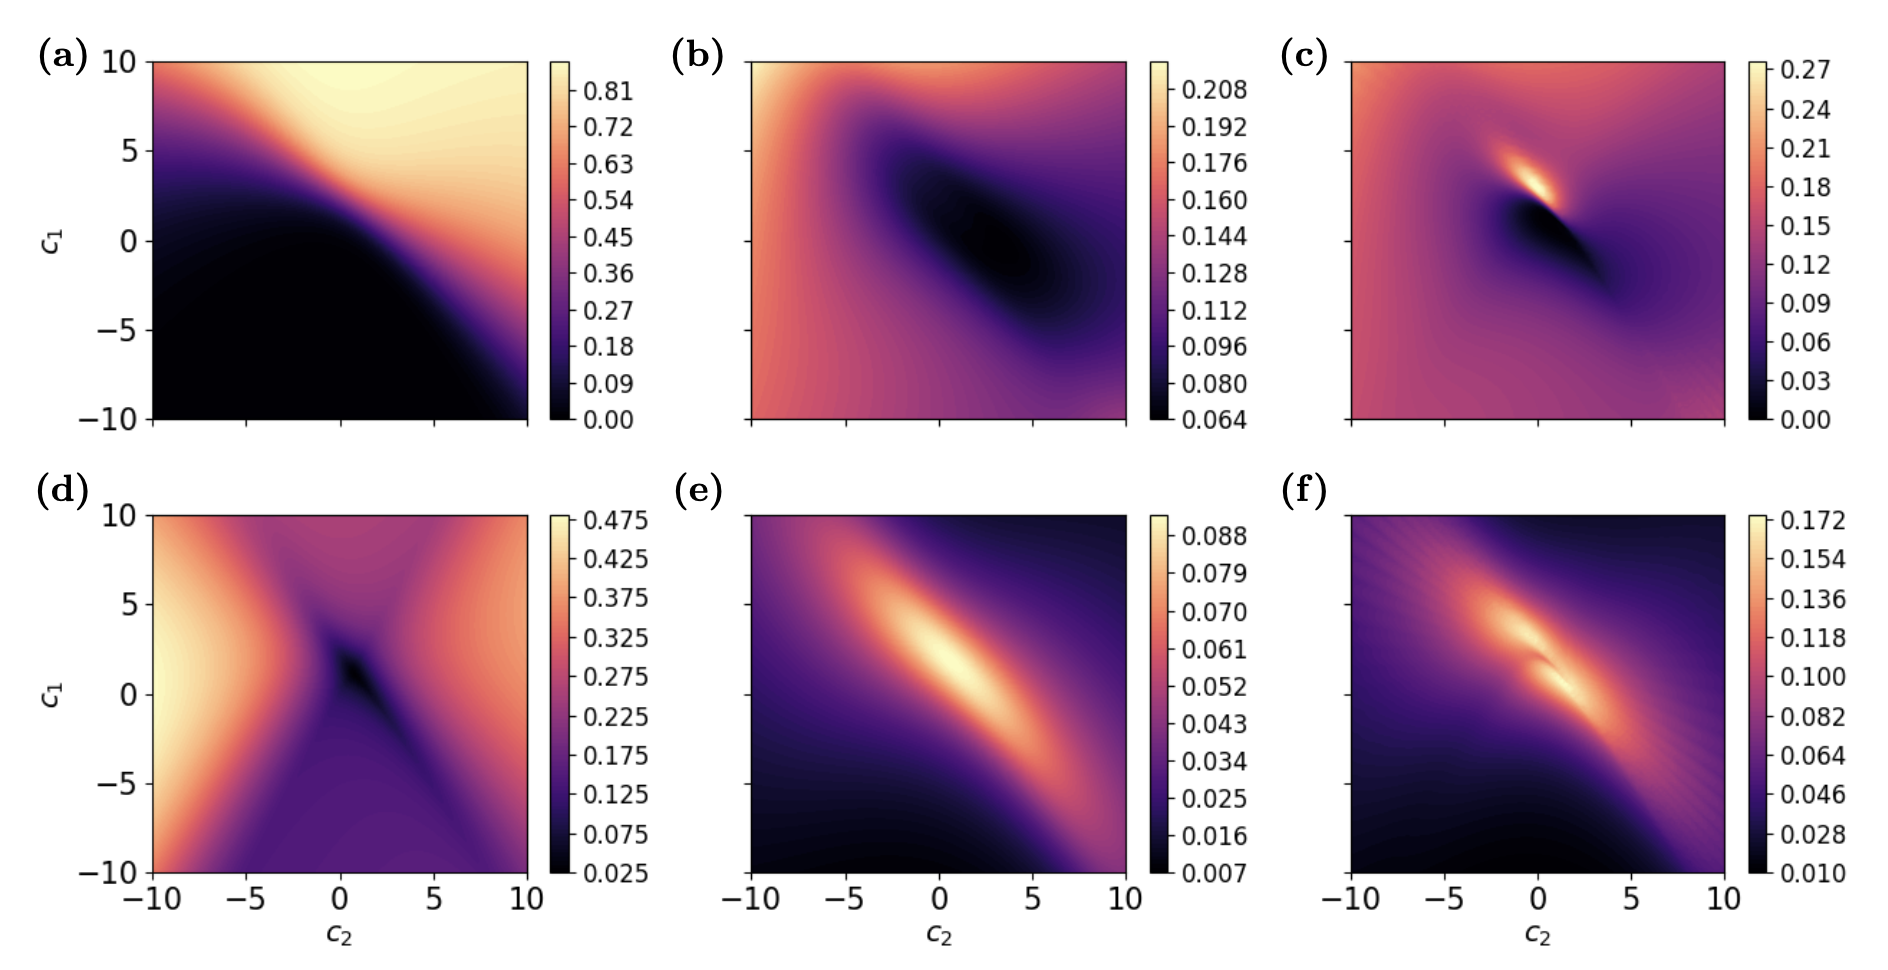
\includegraphics[width=\linewidth]{images/two_spin_contours_integrals.png} \caption[Two-spin annealing contour plots for final state fidelity and AGP integral cost function values.]{Contour plots of fidelity and \acrref{AGP} integral cost function landscapes for two parameters $c_1, c_2 \in [-10, 10]$ for two spin annealing, as discussed in the text. All plots are for total evolution time $\tau = 0.1 h_0^{-1}$. (a)-(c) Plots of fidelity cost function $C_F$ values when (a) \acrref{FO} \acrref{LCD} is applied ($\alpha$ terms), (b) \acrref{SO} \acrref{LCD} $\zeta$ terms are applied and (c) both \acrref{SO} \acrref{LCD} terms $\gamma$ and $\zeta$ are applied as discussed in the text. (d)-(f) show plots of the integral cost function $C_I$ values for (d) the coefficient $\alpha$, $C_{I, \alpha}$ (e) the coefficient $\zeta$, $C_{I, \zeta}$ and (f) sum of the coefficients $\gamma$ and $\zeta$, $C_{I, \gamma + \zeta}$.}\label{fig:two_spin_higher_order}
\end{figure}

\section{Ising chain and omitting LCD pulses}

\begin{figure}[h]
    \centering
    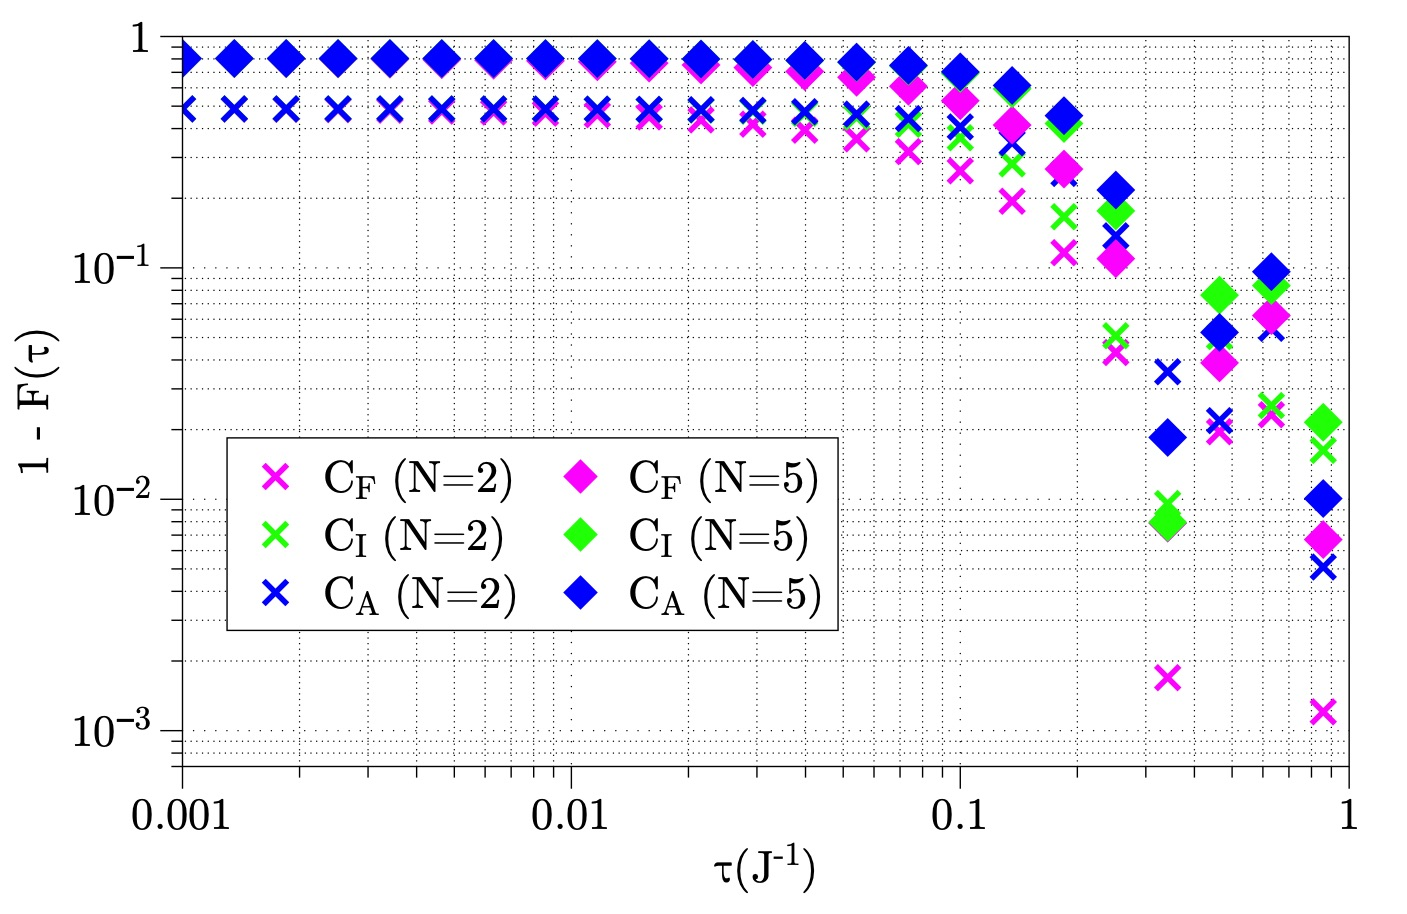
\includegraphics[width=0.8\linewidth]{images/No_cd_higher_order.jpg} \caption[Plot of final state fidelity for the Ising spin chain for different cost functions and no LCD.]{Plot of final state fidelities obtained when optimising for the fidelity cost function (Eq.~\eqref{eq:costfunc_fidelity}, blue), the \acrref{LCD}  }\label{fig:ising_nocd_higher_order}
\end{figure}

\begin{figure}[h]
    \centering
    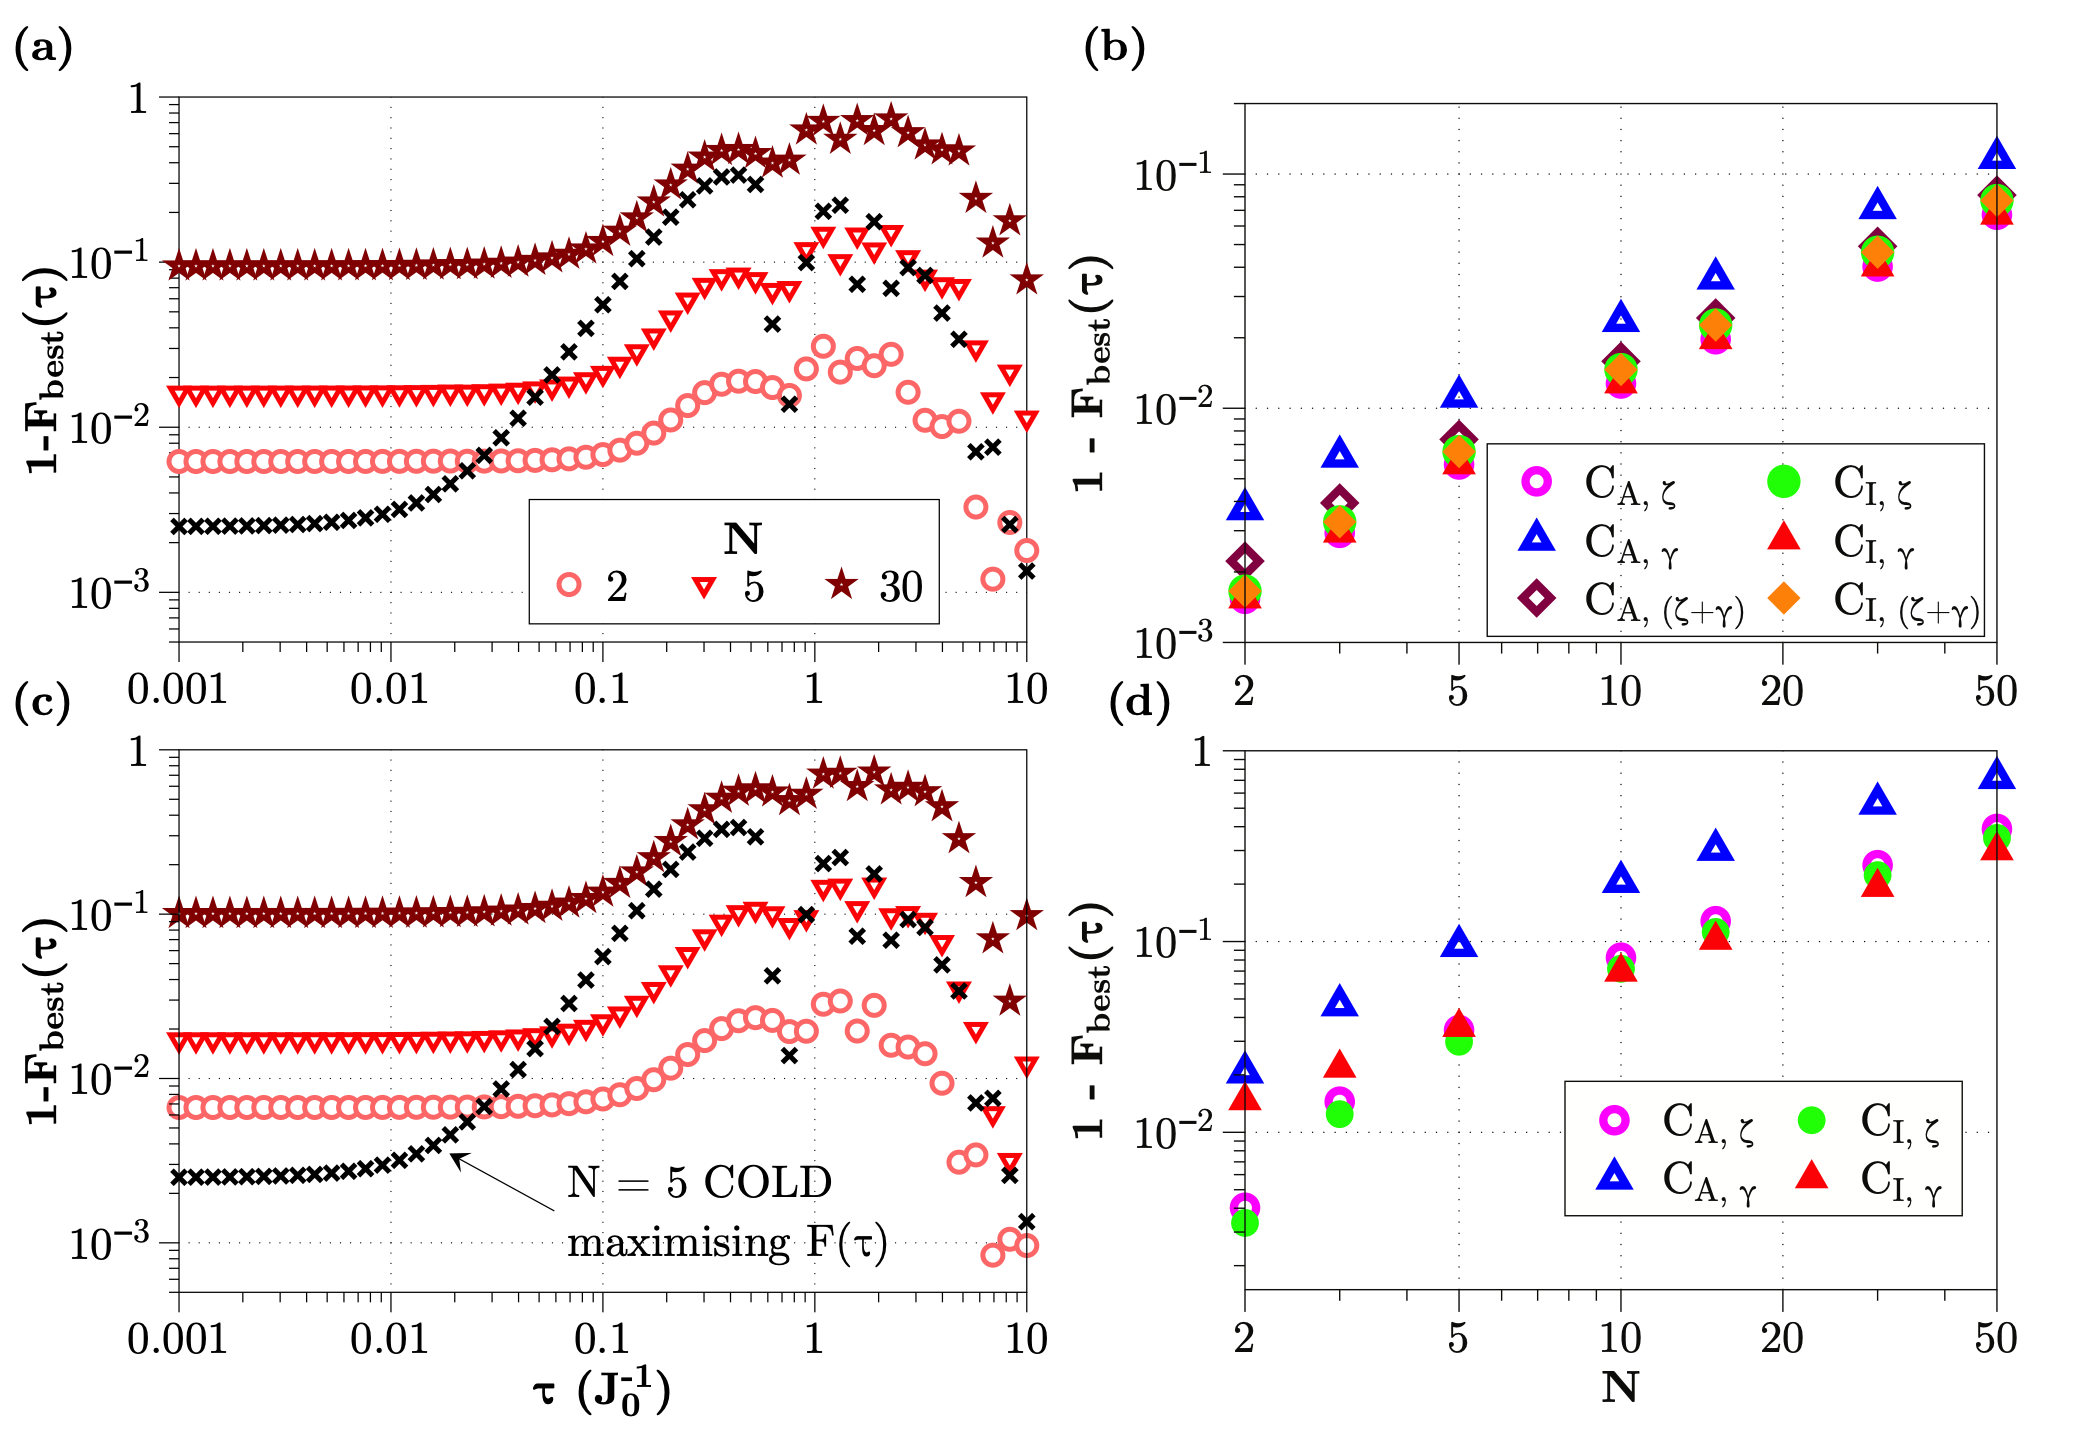
\includegraphics[width=\linewidth]{images/ising_max_int_plots.png} \caption[Plot of final state fidelity for the Ising spin chain for different cost functions with LCD applied.]{}\label{fig:ising_lcd_max_int}
\end{figure}

\section{GHZ states, fidelity and entanglement}

\begin{figure}[t]
    \centering
    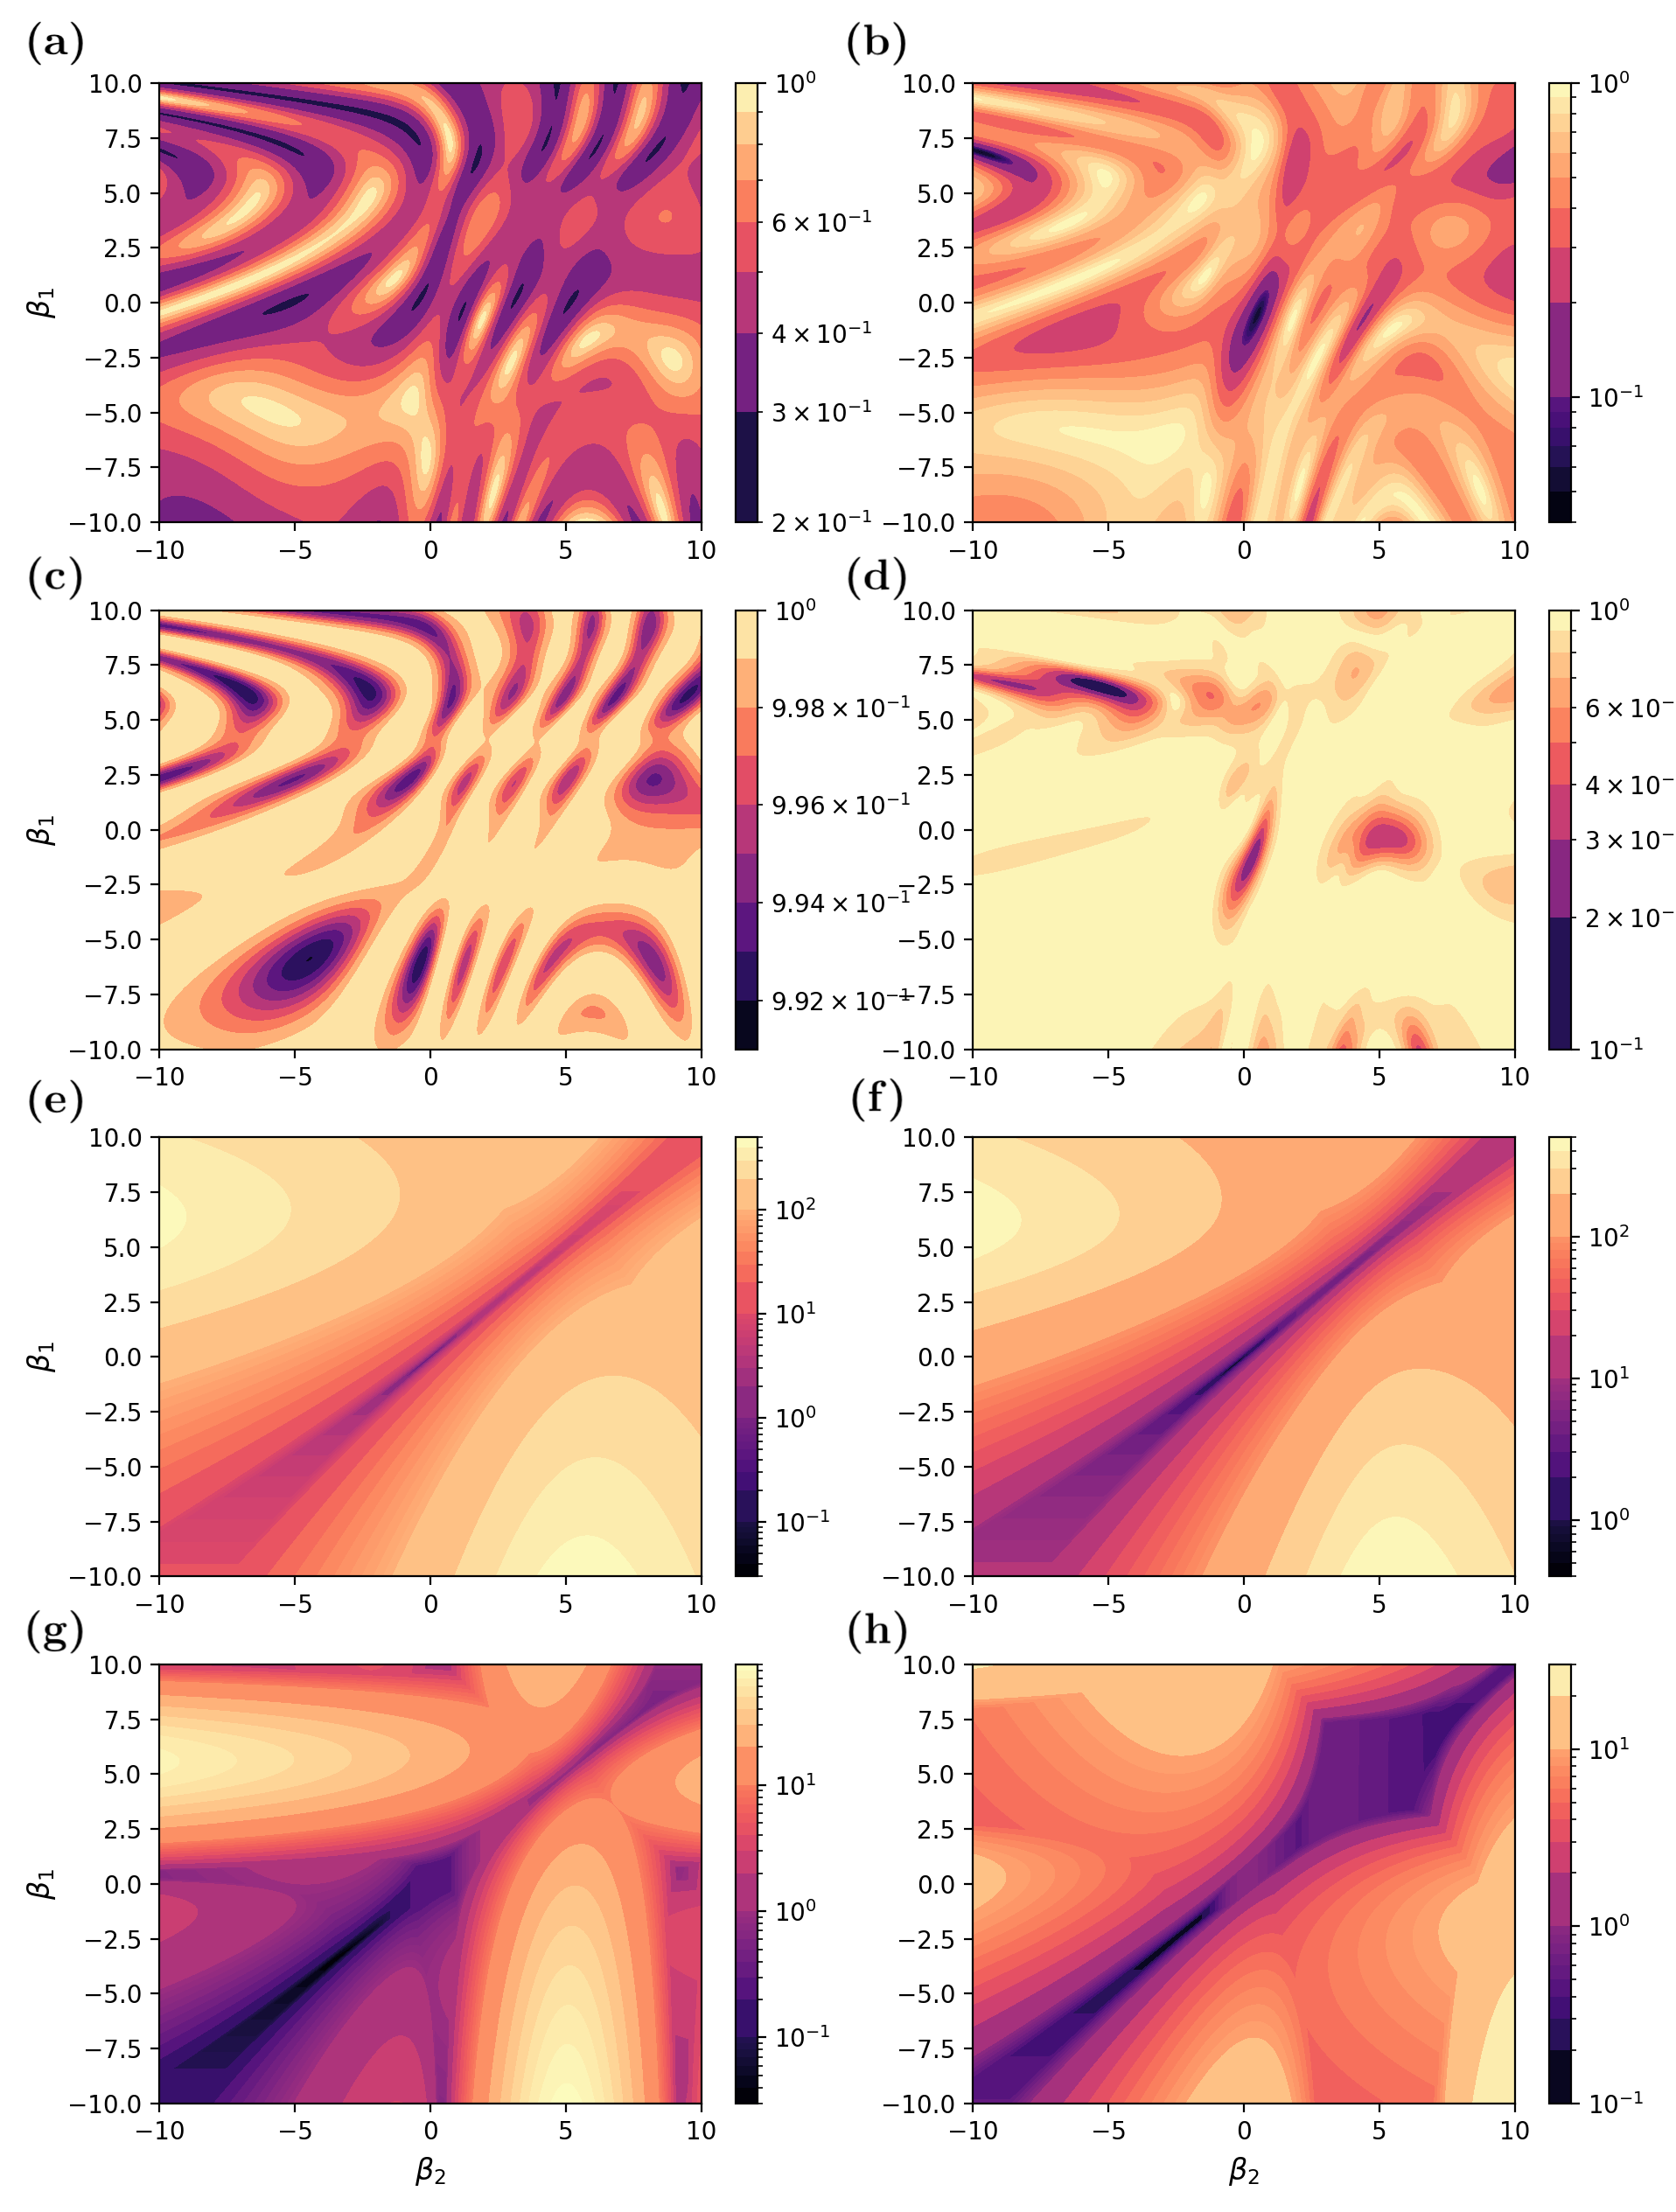
\includegraphics[width=\linewidth]{images/ghz_contour_plots.png} \caption[Contour plots of cost function landscapes for GHZ state preparation in frustrated spin systems.]{Contour plots, $\tau = 0.1 J^{-1}$, \acrref{GRAPE} for parameters $\beta_1$ and $\beta_2$. (a) FO CD infidelity, (b) SO CD infidelity, (c) FO CD $1 - T_3$, (d) SO CD $1 - T_3$, (e) FO CD amps ($\alpha$), (f) SO CD amps ($\alpha$) (g) SO CD amps ($\gamma$) (h) SO CD amps ($\zeta$)}\label{fig:ghz_contours}
\end{figure}